%\documentclass[letterpaper, 12pt]{report}
\documentclass[letterpaper, 11pt]{article}
%\author{Brian Bell}
%\date{2-10-2013}
%\title{Humans as Property in the Early West: \\ Contrasting the Origins and Operation of Russian Serfdom with the Peculiar Instituton of Slavery in the United States.}
%\affiliation{2102055378 \\ HST-104 (10162)}


%\usepackage[dvips]{graphicx}
%\usepackage[pdftex]{graphicx}
\usepackage{graphicx}
%\usepackage[dvipdfmx]{graphicx}
\DeclareGraphicsExtensions{.eps,.pdf,.jpg,.png}

%\usepackage[caption=false,labelfont=sf,textfont=sf,captionskip=5pt]{subfig}

%\DeclareGraphicsRule{.pnXg}{eps}{.bb}{}

\usepackage{achicago}
\usepackage{fullpage}
%\usepackage[top=1in, bottom=1in, left= 1 in, right=1in]{geometry}
%\usepackage[top=1.5in, bottom=1.5in, left=1.5in, right=1in]{geometry}
\usepackage{geometry}

%\usepackage{natbib}
%\usepackage[natbib=true, bibstyle=authoryear, citestyle=authoryear-comp]{biblatex}

% for distance between bib items
\usepackage{bibspacing}
\setlength{\bibitemsep}{1.0\baselineskip plus .05\baselineskip minus .05\baselineskip}

%\usepackage[super,sort&compress]{natbib}

\usepackage{layout}

\usepackage{setspace}


\usepackage[nopar]{lipsum} % for dummy text
\usepackage[american]{babel}
\usepackage[babel]{csquotes}
%\usepackage{natbib}
%\usepackage[notes,natbib,isbn=false,backend=biber]{biblatex-chicago}
%\addbibresource{bibfile.bib}

\usepackage{fancyhdr}

%\fancyhf{}
%\fancyhead[C]{\thepage}
%\pagestyle{fancy}

% redefine the plain pagestyle
%\fancypagestyle{plain}{%
%\fancyhf{} % clear all header and footer fields
%\fancyhead[C]{\thepage} % except the center
%}

%\usepackage{chicago}
%\usepackage{fancyhdr}
\pagestyle{fancy}
%\fancyhead[R]{Humans as Property in the Early West - \thepage}
\fancyhead[R]{\thepage}
\fancyfoot{}
\renewcommand{\headrulewidth}{0pt}
\renewcommand{\footrulewidth}{0pt}


%\newcommand{\HRule}{\rule{\linewidth}{0.25mm}}
\newcommand{\HRule}{\rule{\linewidth}{0mm}}

\doublespacing
%\setlength{\parindent}{0pt}

% 36pt == 0.5in


\setlength{\voffset}{0in}
\setlength{\hoffset}{0in}

\setlength{\marginparpush}{0in}
\setlength{\footskip}{0in}

\setlength{\marginparsep}{0in}
\setlength{\marginparwidth}{0in}

\setlength{\textheight}{578pt}
\setlength{\textwidth}{434pt}



%\setlength{\oddsidemargin}{0.5in}

\setlength{\topmargin}{0in}
\setlength{\headheight}{0in}
\setlength{\headsep}{0.5in}

\setlength{\footnotesep}{24pt}
%\setlength{\skip\footins}{0pt}

\setlength{\parindent}{4em}

%\setlength\bibitemsep{1.5\itemsep}
%\setlength{\bibitemsep}{1.5in}


\begin{document}%\layout
\begin{titlepage}
\begin{center}

\HRule

\textbf{\Huge Machine Learning 101} \\
\bigskip\bigskip\bigskip\bigskip\bigskip\bigskip\bigskip\bigskip\bigskip\bigskip\bigskip
{Group 11: Bide Xu (260711367)}\\
{Mengjia Gu (260790140)}\\
{Robin Luo (260851506)}\\
\bigskip\bigskip\bigskip\bigskip\bigskip\bigskip\bigskip\bigskip\bigskip\bigskip\bigskip
{Course Number: COMP 551}\\
{Course Name: Applied Machine Learning}\\
{\today}

\end{center}
\end{titlepage} 

\clearpage
\setcounter{page}{2}
%\autocite{citekey} just use footnotes!

\singlespacing

\begin{abstract}
Online posts and forums have become increasingly popular in daily use and valuable in marketing support. Hence, prediction on comment popularity is explorable for more applications. This project was purposed to assess the performance of linear regression models for predicting comment popularity on Reddit. Given the pre-crawled dataset, we preprocessed data, extracted features, and built models for both closed-form solution and gradient descent. Not as the theoretical expectation, out experiment results illustrated that, compared to gradient descent method, closed-form solution is better in both runtime and accuracy. Compared models differently implemented with text features, we noticed that involving text content of a comment into models obviously improved the accuracy of prediction on popularity. By adding new input variables like comment text length and average number of words per sentence, we deduced the significance of comment content in prediction of popularity. Some more features like post topic, user community, and image use are considered as potential factors affecting comment popularity, which are not yet evaluated in this project.
\end{abstract}

\section*{Introduction}
Discussion board is frequently used in academic communication, product review and other public message exchange. This variety of information, which serves as a data source of the predicting technique, contributes to commercial development in recommendation system design\cite{rohlin2016popularity}.

Reddit is a classic and popular discussion platform, connecting communities with various topics. This project is proposed to construct and compare linear regression models in purpose of predicting comment popularity on Reddit. We are given some prepared data of selected comments, which still required preprocessing before import into experiments. Three features (children, controversiality, is\_root) and one output variable are directly from the original dataset. Other input variables, such as text features and word counts, were extracted or derived from text content of comments.

We applied two approaches of linear regression models, closed-form solution and gradient descent, to prediction models with and without text features. Although we modified value of hyperparameters in gradient descent and tried to improve performance, the closed-form solution actually runs faster and presents more accurate and stable results. Including richer text features and considering comment length and average words per sentence indeed reduced mean square errors of models and hence improved performance. (With word filters, text features even help more in prediction of comment popularity.)


\section*{Dataset}
The original dataset consists of 12,000 data points in format of dictionary. Each dictionary contains five keys with different types of value. Data in each type of information forms one or more variables in linear regression models. We translated some of them in format better support linear regression models, as described below:

\begin{itemize}
    \item popularity\_score: numeric output variable, larger value means more popular comment
    \item children: non-negative integers indicate number of replies received
    \item controversiality: binary metric, 0 means not controversial and 1 means controversial comment
    \item is\_root: binary, True represents a direct comment instead of being a reply, and contrary for False
    \item text: text content of a comment, which is convert to lower case and split by space, to generate new features
\end{itemize}

Besides the popularity\_score representing how popular each comment is, other information are taken as input variables that may affect prediction results. Text features are drawn from a wordlist of most frequently used words in all given comments. This wordlist contains 160 words ranking by occurrences in text content of comments. We as well count total number of words of comment and average word per sentence in each text value in order to add them as new features improving prediction.

After preparing features, we divided dataset into three parts for different purposes: first 10000 for data training, next 1000 as a validation set, and last 1000 to test model. Considered the limitation of data source, out project may lose accuracy lacking data of more features like post topics and timeline. Failures in measuring popularity score could also lead to missing objectiveness and reliability of our data source. Moreover, user preference is always difficult to detect, especially that Reddit targets on public audience with various backgrounds.


\section*{cite and figure}

%work\cite[pp. 3]{rohlin2016popularity} of ``The doctrine of the sword''

%\begin{figure}
%  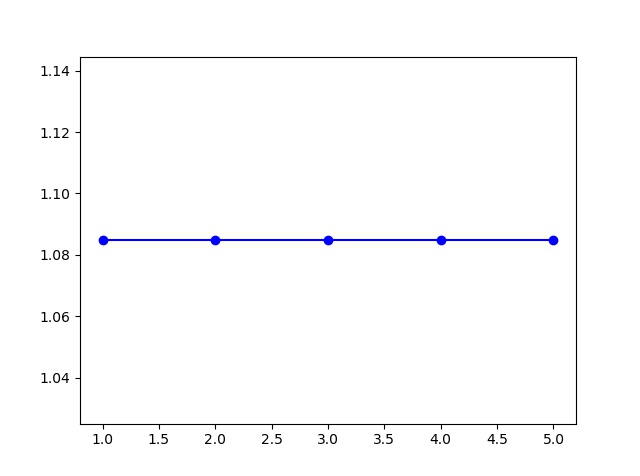
\includegraphics[width=\linewidth]{fig/pic1.jpg}
%  \caption{Relationship among }
%  \label{fig:relation1}
%\end{figure}


\begin{figure}[!t]
  %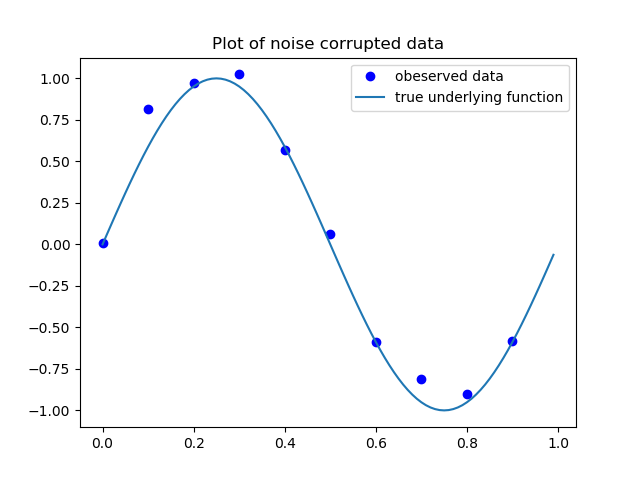
\includegraphics[width=0.28\textwidth]{fig/figure_3.png}
  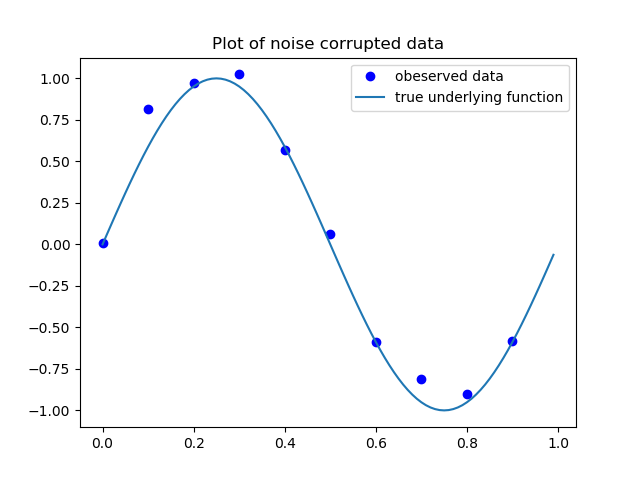
\includegraphics[width=\linewidth]{fig/figure_3.png}
  \caption{Relationship among }
  \label{fig:relation1}
\end{figure}

%\begin{figure}[!b]
%  \centering
%  \setlength{\fboxrule}{0.0pt}
%  \setlength{\fboxsep}{0.0cm}
%  \subfloat[]{\fbox{\label{fig:fg-Low-18x18-PD}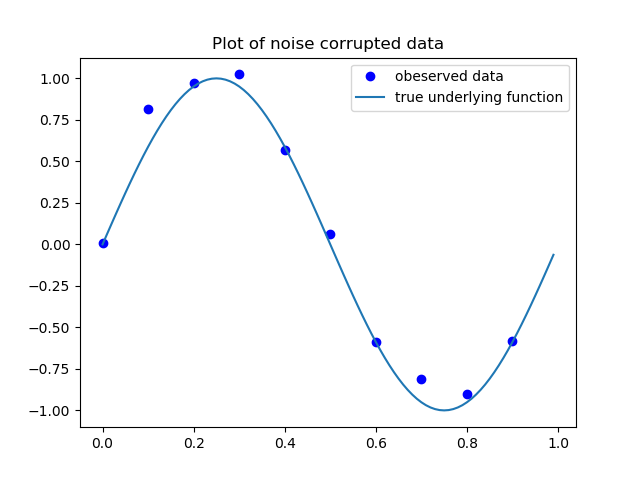
\includegraphics[angle=0, width=0.28\textwidth]{fig/figure_3.png}}}
%  \subfloat[]{\fbox{\label{fig:fg-High-23x23-PD}\includegraphics[angle=0, width=0.28\textwidth]{}}}
%  \caption{Trend for }\label{fig:fg-ImprovementPD}
%\end{figure}

%\begin{figure}[!t]
%  \centering
%  \setlength{\fboxrule}{0.1pt}
%  \setlength{\fboxsep}{0.0cm}
%  \subfloat[]{\fbox{\label{fig:fg-TC-DELETE2}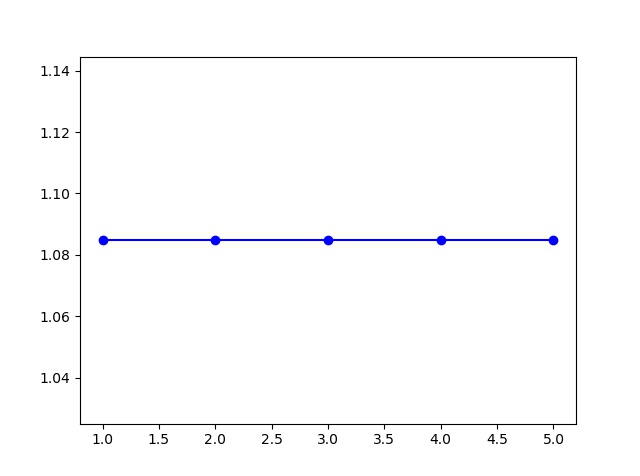
\includegraphics[angle=0, width=0.22\textwidth]{fig/pic1.jpg}}}
%  \subfloat[]{\fbox{\label{fig:fg-TC-DELETE4}\includegraphics[angle=0, width=0.22\textwidth]{}}}\\
%  \subfloat[]{\fbox{\label{fig:fg-TC-ADD2}\includegraphics[angle=0, width=0.22\textwidth]{}}}
%  \subfloat[]{\fbox{\label{fig:fg-TC-ADD4}\includegraphics[angle=0, width=0.22\textwidth]{}}}
%  \caption{Procedure for }\label{fig:fg-delete-and-add}
%\end{figure}

\section*{Results}


\subsection*{Closed-Form Solution v.s. Gradient Descent}

Simply with non\---text features directly extracted from dataset, closed-form solution without extra hyperparameter stands out for its stability and smaller mean square errors of both training and validation sets.Besides input variables, three hyperparameters affected results by gradient descent. Lowering learning rate took longer time to reduce mean square errors, while increasing elapsed\_time ended experiment before reaching small mean square errors. Although the third hyperparameter distance\_power\_rate was added to address some balance between speed and accuracy, the model using gradient descent still took longer time than the one with closed-form solution.

\subsection*{Text Features}

Implemented with the closed\---form solution, models using more text features from the wordlist took longer time to present lower mean square errors on both training and validation sets. After applying the word filters to remove punctuations and stopping words, mean square errors even dropped to some lower value. Statistic data support this result in Figure 1.


\subsection*{New Features}
Both total length of comment and average number of words per sentence in each comment reduced the mean square errors of linear regression models in predicting comment popularity. See Figure 2.

\section*{Discussion and Conclusion}

This project indicated better results of linear regression models with closed-form solution than which with gradient descent, which against the theoretical suggestion of better performance by gradient descent. One possible explanation is that small size of dataset, requiring only few operations, cannot reflect the advantage of gradient descent in dealing with huge data and complex operations.

More and better filtered text features improves the prediction accuracy. Other features derived from text data, like comment length and word counts per sentence, better predict the comment popularity as well. Newly added features are also related to text content of comments. Therefore, text content significantly affects the popularity of a comment. Meanwhile, more text features take models longer time to run experiments.

More features in reality should be considered as important variables affecting how popular a comment on Reddit is. The idea of predicting comment popularity facilitates in technical development in commercial area, especially through improving recommendation systems.



\nocite{*}

\bibliographystyle{achicago}



\begingroup

    %\setlength{\bibsep}{10pt}

    \setstretch{1}
    \bibliography{bibfile}


\endgroup
%\renewcommand{\baselinestretch}{2.1}
\renewcommand{\thepage}{}

%\bibliography{bibfile}

\section*{Contribution Statement}

All members brainstormed for data preparation, feature extraction, and model construction.
\begin{itemize}
    \item Bide Xu: main python coding
    \item Robin Luo: models improvement and graph plotting
    \item Mengjia Gu: results test and summarize write-up
\end{itemize}All participated in whole progress and learnt through this project.

%\setlength{\bibitemsep}{1.5itemsep}
%\setlength{\bibnamesep}{1.5itemsep}
%\setlength{\bibinitsep}{1.5itemsep}



%\pagestyle{fancy}
%\fancyhead[R]{\thebibliography}
%\fancyfoot{}
%\renewcommand{\headrulewidth}{0pt}
%\renewcommand{\footrulewidth}{0pt}



\end{document} 